\section{An overview of document preparation systems}
	A \emph{document preparation system} is any software that is used to \emph{create}, \emph{edit}, \emph{format} and \emph{structure} text for printing or digital viewing. Rather than just acting as digital typewriters, these systems manage the entire lifecycle of a document.
	
	There are four main functions of a document preparation system:
	\begin{enumerate}[a)]
		\item \emph{Content ingestion}, which means providing an interface via which the user can input and edit text.
		\item \emph{Structural tagging}, which refers to defining what the text is, e.g. chapter title, section title, footnote or a caption.
		\item \emph{Stylistic rendering}, which indicates the application of typefaces, margins, line spacing and alignment of structural elements.
		\item \emph{Output compilation}, which signifies the conversion of the working file into a printed sheet, or a ubiquitous format like PDF, HTML or EPUB.
	\end{enumerate}
	
	\subsection{Categories of document preparation systems}
		Document preparation systems can be broadly classified into two categories:
		\begin{enumerate}
			\item \textbf{Word processing software:} Such software are designed for general-purpose writing, editing, and basic layout of everyday documents like letters, reports and memos.
			\begin{itemize}
				\item Typically, the interface is WYSIWYG which stands for \emph{What You See Is What You Get}. This means that text and formatting appear on the screen as they will approximately look when printed.
				\item Elements like images and tables are usually anchored directly to the text flow and move down the page as you type or add content.
				\item The formatting approach relies heavily on direct manual formatting (such as changing font sizes, italicising or spacing on the fly) or applying predefined template styles.
				\item Some examples are Microsoft Word, Google Docs and LibreOffice Writer.
			\end{itemize}
			
			\item \textbf{Typesetting software:} Such software are designed for publication-grade document composition, strict typographic control (such as kerning, hyphenation, and line-breaking algorithms) and complex scientific or multi-column layouts.
			\begin{itemize}
				\item The interface is often markup-based. Thie means that writing plain text mixed with structural code or commands that get compiled into a final PDF, rather than a direct visual editor.
				\item Automated algorithms are used to manage images and tables, page breaks, mathematical formulae and bibliographic references without manual nudging.
				\item The formatting approach strictly separates content from presentation, i.e the user focuses on the content and its semantics (e.g., heading, theorem, citation etc.), while the underlying algorithm applies exact, consistent formatting rules.
				\item Some examples are \LaTeX, Typst and Troff.
			\end{itemize}
		\end{enumerate}
		
	\subsection{Separation of content and formatting in scientific documentation}
		In scientific documentation, enabling the separation of content (e.g. text, data, structure) and formatting (e.g. font, margins, layout) allows the author to shift one's focus from presentation to substance. Such an approach is provided by \LaTeX, with the following advantages:
		\begin{enumerate}[a)]
			\item Authors write in plain text using semantic tags to define structural elements, while the software handles the visual rendering in the background. Consequently, the author can spend their time refining arguments, data accuracy and prose, rather than struggling with erratic margins, font consistency or manual line breaks.
			\item Global style files control the entire document's appearance. So any formatting changes instantly updates the entire manuscript consistently, thereby minimising human error.
			\item Scientific documents rely heavily on interconnected data. When content is decoupled from style, the system can dynamically manage complex modules without manual intervention.
			\begin{enumerate}[i.]
				\item Mathematical equations are rendered using precise algorithmic typesetting that maintain correct spacing and symbol scales regardless of surrounding text adjustments.
				\item Citations, figures, tables and equations are linked to logical labels. If a figure is moved or added, the system automatically renumbers every reference throughout the document.
				\item Bibliographies are generated directly from a central database file. Thereby the system parses the database and formats the citations perfectly according to the required style guide.
			\end{enumerate}
			\item Submitting a paper to a different journal often requires an entirely new layout. With a separated system, authors do not need to manually reformat headers, margins or citation styles. They simply swap out the publisher's template file or package declaration, and the document automatically reshapes itself to meet the new submission guidelines.
			\item Plain-text content files are exceptionally lightweight and compatible with standard version control systems like Git. Unlike proprietary binary files such as DOCX, plain-text documents allow co-authors to view precise line-by-line changes, merge collaborative edits seamlessly and track the manuscript's evolution without the risk of file corruption.
		\end{enumerate}
		
	\subsection{What is \LaTeX?}
		\LaTeX\ is free, open source, markup-based software for typesetting documents. In other words, it is a document preparation system. \LaTeX\ was initially developed in the 1980's by Leslie Lamport, based on Donald Knuth's \TeX\ typesetting engine.
		
		\subsubsection{Benefits of \LaTeX}
			\LaTeX\ is best suited for scientific and technical documents, because of its superior typesetting of mathematical formulae, consistency of high-quality output, and ease of handling large and complex documents. Some of the benefits of \LaTeX\ are listed below:
			\begin{enumerate}
				\item Ability for automatic numbering of equations, tables, figures and sections.
				\item Capabilities for cross-referencing labels.
				\item Automatic generation of lists of contents, figures, tables, indexes, glossaries and bibliography.
				\item Versatility of document types that can be prepared, such as articles, reports, letters, books and presentation slides.
				\item Flexibility in terms of availability of various templates for a given type of document.
				\item Portability in terms of source files being compatible across systems and output being device-independent.
				\item Scalability in terms of handling documents of any length without performance degradation.
				\item Support from a massive online community of other \LaTeX\ users from all over the world.
			\end{enumerate}
			
		\subsubsection{Working with \LaTeX}
			There are two ways of working with \LaTeX:
			\begin{enumerate}[A.]
				\item Installing the \LaTeX\ compiler and an optional IDE on one's own computer.
				\begin{itemize}
					\item Examples of \LaTeX\ compilers are \href{https://miktex.org/}{MikTeX} and \href{https://www.tug.org/texlive/}{TeXLive}.
					\item Examples of IDEs are \href{https://www.texstudio.org/}{TeXstudio} and \href{https://www.xm1math.net/texmaker/}{TeXmaker}.
					\item \emph{Note}: Even though installing \LaTeX\ is recommended, it may take up about 8 GB space on the hard drive and at least 2 hours for the installation.
				\end{itemize}
				
				\item Using \LaTeX\ online \emph{in the cloud}, with the minimum requirement being a browser on an internet-connected device.
				\begin{itemize}
					\item Examples of online \LaTeX\ services are \href{https://www.overleaf.com}{Overleaf} and \href{https://app.inscrive.io}{Inscrive}.
					\item \emph{Note}: Even though Overleaf is free to use, it has an upper limit on the compilation time, and this limit can be raised with a paid subscription. So for a free account, with an increase in the complexity of the document, the chances of the document not compiling also increases.
				\end{itemize}
			\end{enumerate}
			
	\subsection{Working with \LaTeX\ on Overleaf}
		Overleaf is an excellent starting point for someone who is getting started with using \LaTeX\ without getting overwhelmed with the hassle of installation.
		
		Some of the benefits of Overleaf are as follows:
		\begin{itemize}
			\item It can be accessed on any device, such as PC, laptop, tablet or smartphone.
			\item It can be accessed from a locked-in work computer, where one is not allowed to install any software.
			\item One can access one's files on any device simply by logging in with one's password.
			\item One can collaborate with others to work on the same project.
			\item It provides a real-time view of the PDF output.
			\item It allows one to annotate the \LaTeX\ code with comments and replies.
		\end{itemize}
		
		\subsubsection{Creating a \LaTeX\ project online}
			\begin{enumerate}[I.]
				\item For a one-time registration, either click on \verb|Register| on the Overleaf home page or visit \url{https://www.overleaf.com/register}. Enter an email address and choose a password.
				
				\item To log in to Overleaf, either click on \verb|Login| on the Overleaf home page or visit \url{https://
				www.overleaf.com/login}.
				
				\begin{figure}[h!]
					\centering
					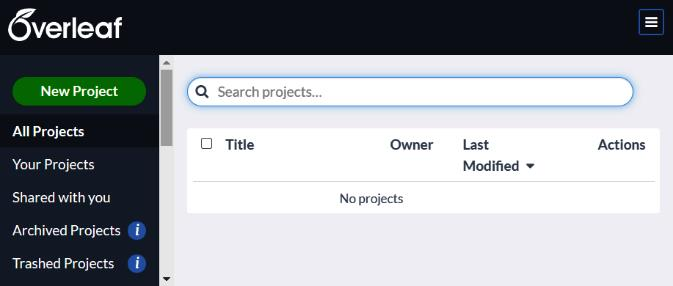
\includegraphics[width=0.7\textwidth]{figures/fig_overleaf-new-project.jpg}
				\end{figure}
				
				\item To create a new project, click the \verb|New Project| button. A drop-down list will appear, where one can choose to have a blank project or one based on a template. For now, we just choose \verb|Blank Project|.
				
				\item We enter a name for the project and Overleaf creates one with the bare minimum of code.
				
				\begin{figure}[h!]
					\centering
					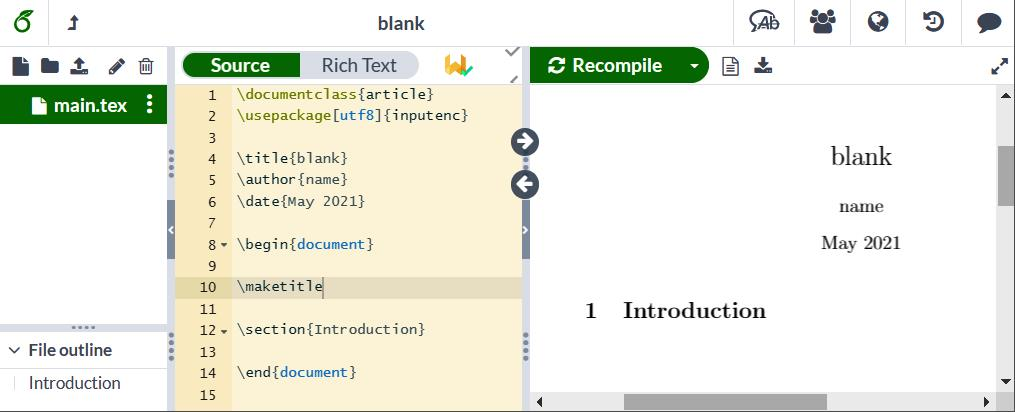
\includegraphics[width=0.8\textwidth]{figures/fig_overleaf-blank-project.jpg}
				\end{figure}
				
				\newpage
				\item When any new changes are made to the project, we can view their effect on the output PDF by clicking on the \verb|Recompile| button or pressing \verb|Ctrl+S|. Enabling the \verb|Auto Compile| option in the drop-down menu will ensure that the document recompiles automatically while one is typing.
				
				\begin{figure}[h!]
					\centering
					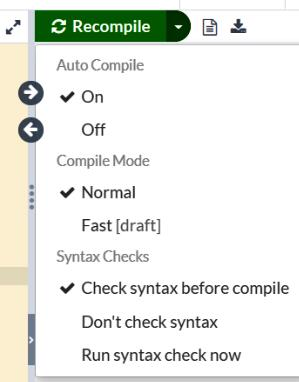
\includegraphics[width=0.4\textwidth]{figures/fig_overleaf-recompile.jpg}
				\end{figure}
				
			\end{enumerate}